\documentclass{standalone}
\usepackage{tikz}
\usetikzlibrary{patterns, positioning}


\begin{document}
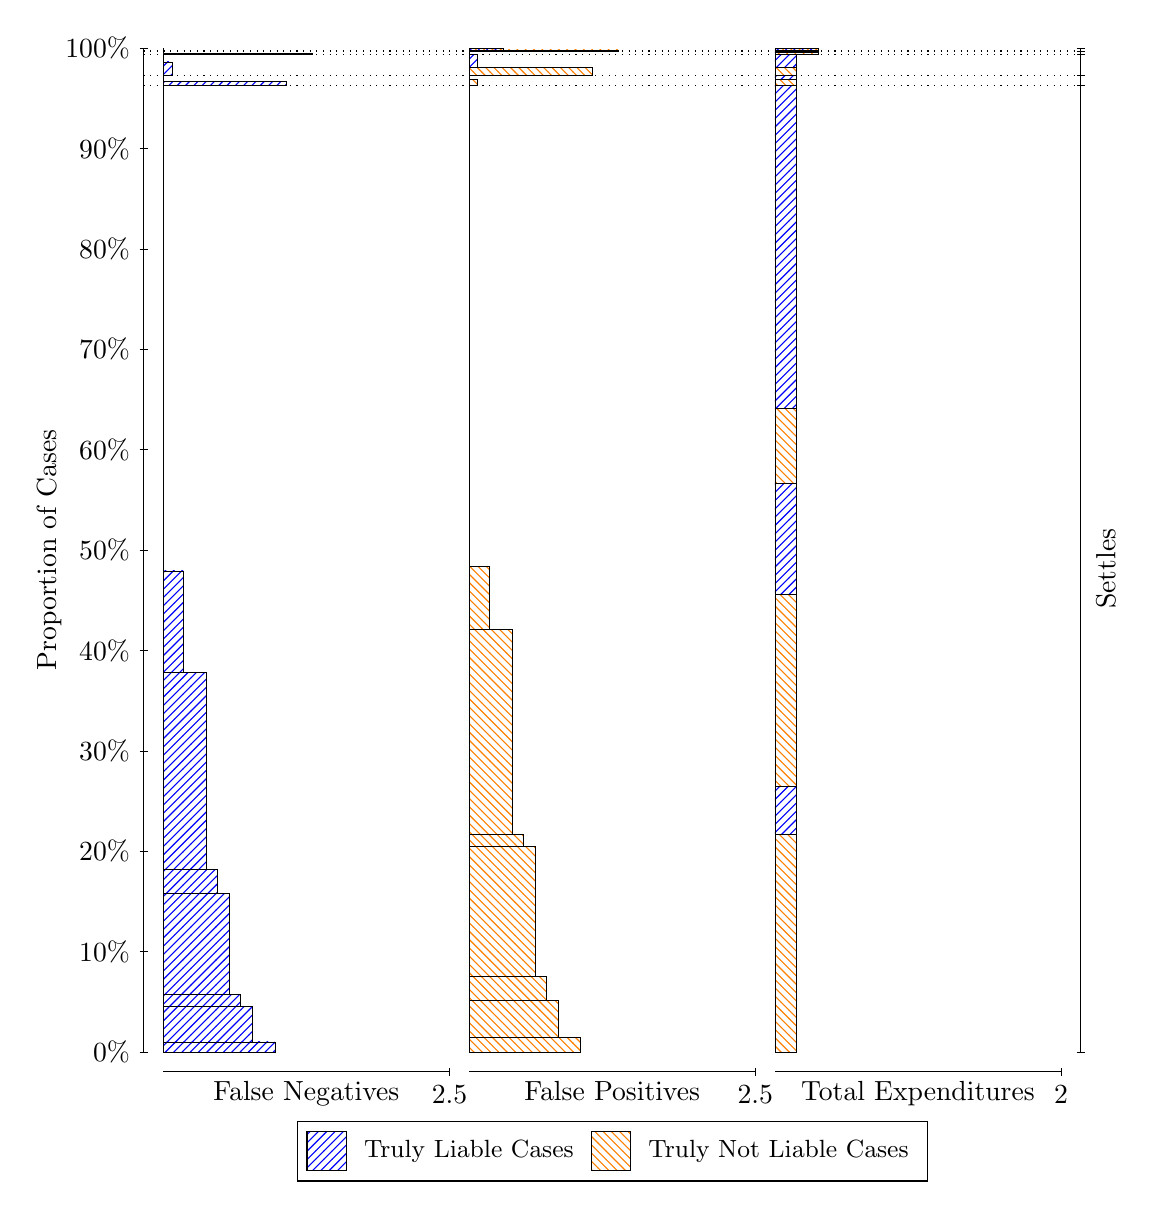
\begin{tikzpicture}
\draw[black, very thin] (1.5,1.75) -- (1.5,14.5);
\node[rotate=90, text=black, anchor=center] at (0.3, 8.125) {Proportion of Cases};
\draw[black, very thin] (1.45,1.75) -- (1.55,1.75);
\node[text=black, anchor=east] at (1.45, 1.75) {0\%};
\draw[black, very thin] (1.45,3.025) -- (1.55,3.025);
\node[text=black, anchor=east] at (1.45, 3.025) {10\%};
\draw[black, very thin] (1.45,4.3) -- (1.55,4.3);
\node[text=black, anchor=east] at (1.45, 4.3) {20\%};
\draw[black, very thin] (1.45,5.575) -- (1.55,5.575);
\node[text=black, anchor=east] at (1.45, 5.575) {30\%};
\draw[black, very thin] (1.45,6.85) -- (1.55,6.85);
\node[text=black, anchor=east] at (1.45, 6.85) {40\%};
\draw[black, very thin] (1.45,8.125) -- (1.55,8.125);
\node[text=black, anchor=east] at (1.45, 8.125) {50\%};
\draw[black, very thin] (1.45,9.4) -- (1.55,9.4);
\node[text=black, anchor=east] at (1.45, 9.4) {60\%};
\draw[black, very thin] (1.45,10.675) -- (1.55,10.675);
\node[text=black, anchor=east] at (1.45, 10.675) {70\%};
\draw[black, very thin] (1.45,11.95) -- (1.55,11.95);
\node[text=black, anchor=east] at (1.45, 11.95) {80\%};
\draw[black, very thin] (1.45,13.225) -- (1.55,13.225);
\node[text=black, anchor=east] at (1.45, 13.225) {90\%};
\draw[black, very thin] (1.45,14.5) -- (1.55,14.5);
\node[text=black, anchor=east] at (1.45, 14.5) {100\%};

\draw[black, very thin] (13.4,1.75) -- (13.4,14.5);
\draw[black, very thin] (13.35,1.75) -- (13.45,1.75);
\node[anchor=west] at (13.35, 1.75) {};
\draw[black, very thin] (13.35,14.023) -- (13.45,14.023);
\node[anchor=west] at (13.35, 14.023) {};
\draw[black, very thin] (13.35,14.154) -- (13.45,14.154);
\node[anchor=west] at (13.35, 14.154) {};
\draw[black, very thin] (13.35,14.419) -- (13.45,14.419);
\node[anchor=west] at (13.35, 14.419) {};
\draw[black, very thin] (13.35,14.462) -- (13.45,14.462);
\node[anchor=west] at (13.35, 14.462) {};
\draw[black, very thin] (13.35,14.5) -- (13.45,14.5);
\node[anchor=west] at (13.35, 14.5) {};

\draw[black, very thin, pattern color=blue, pattern=north east lines] (1.75,1.75) rectangle (3.167,1.877);
\draw[black, very thin, pattern color=blue, pattern=north east lines] (1.75,1.877) rectangle (2.8763,2.3326);
\draw[black, very thin, pattern color=blue, pattern=north east lines] (1.75,2.3326) rectangle (2.731,2.486);
\draw[black, very thin, pattern color=blue, pattern=north east lines] (1.75,2.486) rectangle (2.5857,3.7635);
\draw[black, very thin, pattern color=blue, pattern=north east lines] (1.75,3.7635) rectangle (2.4403,4.0703);
\draw[black, very thin, pattern color=blue, pattern=north east lines] (1.75,4.0703) rectangle (2.295,6.5682);
\draw[black, very thin, pattern color=blue, pattern=north east lines] (1.75,6.5682) rectangle (2.0043,7.8603);
\draw[black, very thin, pattern color=orange, pattern=north west lines] (1.75,7.8603) rectangle (1.75,14.023);
\draw[black, very thin, pattern color=blue, pattern=north east lines] (1.75,14.023) rectangle (3.3123,14.08);
\draw[black, very thin, pattern color=orange, pattern=north west lines] (1.75,14.08) rectangle (1.75,14.154);
\draw[black, very thin, pattern color=blue, pattern=north east lines] (1.75,14.154) rectangle (1.859,14.324);
\draw[black, very thin, pattern color=orange, pattern=north west lines] (1.75,14.324) rectangle (1.75,14.419);
\draw[black, very thin, pattern color=blue, pattern=north east lines] (1.75,14.419) rectangle (3.6393,14.433);
\draw[black, very thin, pattern color=orange, pattern=north west lines] (1.75,14.433) rectangle (1.75,14.462);
\draw[black, very thin, pattern color=orange, pattern=north west lines] (1.75,14.462) rectangle (1.75,14.475);
\draw[black, very thin, pattern color=blue, pattern=north east lines] (1.75,14.475) rectangle (1.75,14.5);
\draw[black, very thin, pattern color=orange, pattern=north west lines] (5.6333,1.75) rectangle (7.0503,1.9338);
\draw[black, very thin, pattern color=orange, pattern=north west lines] (5.6333,1.9338) rectangle (6.7597,2.4029);
\draw[black, very thin, pattern color=orange, pattern=north west lines] (5.6333,2.4029) rectangle (6.6143,2.7097);
\draw[black, very thin, pattern color=orange, pattern=north west lines] (5.6333,2.7097) rectangle (6.469,4.3605);
\draw[black, very thin, pattern color=orange, pattern=north west lines] (5.6333,4.3605) rectangle (6.3237,4.5139);
\draw[black, very thin, pattern color=orange, pattern=north west lines] (5.6333,4.5139) rectangle (6.1783,7.1198);
\draw[black, very thin, pattern color=orange, pattern=north west lines] (5.6333,7.1198) rectangle (5.8877,7.9131);
\draw[black, very thin, pattern color=blue, pattern=north east lines] (5.6333,7.9131) rectangle (5.6333,14.023);
\draw[black, very thin, pattern color=orange, pattern=north west lines] (5.6333,14.023) rectangle (5.7423,14.097);
\draw[black, very thin, pattern color=blue, pattern=north east lines] (5.6333,14.097) rectangle (5.6333,14.154);
\draw[black, very thin, pattern color=orange, pattern=north west lines] (5.6333,14.154) rectangle (7.1957,14.25);
\draw[black, very thin, pattern color=blue, pattern=north east lines] (5.6333,14.25) rectangle (5.7423,14.419);
\draw[black, very thin, pattern color=orange, pattern=north west lines] (5.6333,14.419) rectangle (5.6333,14.448);
\draw[black, very thin, pattern color=blue, pattern=north east lines] (5.6333,14.448) rectangle (5.6333,14.462);
\draw[black, very thin, pattern color=orange, pattern=north west lines] (5.6333,14.462) rectangle (7.5227,14.475);
\draw[black, very thin, pattern color=blue, pattern=north east lines] (5.6333,14.475) rectangle (6.0693,14.5);
\draw[black, very thin, pattern color=orange, pattern=north west lines] (9.5167,1.75) rectangle (9.7892,4.5092);
\draw[black, very thin, pattern color=blue, pattern=north east lines] (9.5167,4.5092) rectangle (9.7892,5.1182);
\draw[black, very thin, pattern color=orange, pattern=north west lines] (9.5167,5.1182) rectangle (9.7892,7.5624);
\draw[black, very thin, pattern color=blue, pattern=north east lines] (9.5167,7.5624) rectangle (9.7892,8.9669);
\draw[black, very thin, pattern color=orange, pattern=north west lines] (9.5167,8.9669) rectangle (9.7892,9.9266);
\draw[black, very thin, pattern color=blue, pattern=north east lines] (9.5167,9.9266) rectangle (9.7892,14.023);
\draw[black, very thin, pattern color=orange, pattern=north west lines] (9.5167,14.023) rectangle (9.7892,14.097);
\draw[black, very thin, pattern color=blue, pattern=north east lines] (9.5167,14.097) rectangle (9.7892,14.154);
\draw[black, very thin, pattern color=orange, pattern=north west lines] (9.5167,14.154) rectangle (9.7892,14.25);
\draw[black, very thin, pattern color=blue, pattern=north east lines] (9.5167,14.25) rectangle (9.7892,14.419);
\draw[black, very thin, pattern color=orange, pattern=north west lines] (9.5167,14.419) rectangle (10.062,14.448);
\draw[black, very thin, pattern color=blue, pattern=north east lines] (9.5167,14.448) rectangle (10.062,14.462);
\draw[black, very thin, pattern color=orange, pattern=north west lines] (9.5167,14.462) rectangle (10.062,14.475);
\draw[black, very thin, pattern color=blue, pattern=north east lines] (9.5167,14.475) rectangle (10.062,14.5);
\draw[black, dotted] (1.5,14.023) -- (13.4,14.023);
\draw[black, dotted] (1.5,14.154) -- (13.4,14.154);
\draw[black, dotted] (1.5,14.419) -- (13.4,14.419);
\draw[black, dotted] (1.5,14.462) -- (13.4,14.462);
\draw[black, very thin] (1.75,1.5) -- (5.3833,1.5);
\node[text=black, anchor=north] at (3.5667, 1.5) {False Negatives};
\draw[black, very thin] (5.3833,1.45) -- (5.3833,1.55);
\node[text=black, anchor=north] at (5.3833, 1.45) {2.5};

\draw[black, very thin] (5.6333,1.5) -- (9.2667,1.5);
\node[text=black, anchor=north] at (7.45, 1.5) {False Positives};
\draw[black, very thin] (9.2667,1.45) -- (9.2667,1.55);
\node[text=black, anchor=north] at (9.2667, 1.45) {2.5};

\draw[black, very thin] (9.5167,1.5) -- (13.15,1.5);
\node[text=black, anchor=north] at (11.333, 1.5) {Total Expenditures};
\draw[black, very thin] (13.15,1.45) -- (13.15,1.55);
\node[text=black, anchor=north] at (13.15, 1.45) {2};

\node[text=black, centered, rotate=90] at (13.72, 7.8867) {Settles};





\draw (7.449999999999999,1.5) node[draw=none] (baseCoordinate) {};
\begin{scope}[align=center]
        \matrix[scale=0.5, draw=black, below=0.5cm of baseCoordinate, nodes={draw}, column sep=0.1cm]{
            \node[rectangle, draw, minimum width=0.5cm, minimum height=0.5cm, pattern color=blue, pattern=north east lines] {}; &
            \node[draw=none, font=\small, text=black] (B) {Truly Liable Cases}; &
            \node[rectangle, draw, minimum width=0.5cm, minimum height=0.5cm, pattern color=orange, pattern=north west lines] {}; &
            \node[draw=none, font=\small, text=black] (B) {Truly Not Liable Cases}; \\
            };
\end{scope}

\end{tikzpicture}
\end{document}